% Template: http://www.acm.org/sigs/publications/proceedings-templates#aL2 
% 
\documentclass{icn/sig-alternate-2012} % {proc}

\usepackage{amsmath}    % need for subequations
\usepackage{graphicx}   % need for figures
\usepackage{verbatim}   % useful for program listings
\usepackage{color}      % use if color is used in text
\usepackage{subfigure}  % use for side-by-side figures
\usepackage{hyperref}   % use for hypertext links, including those to external documents and URLs
\usepackage{url}
\usepackage{multicol}
\usepackage{textcomp}
%\usepackage{caption}  %% supported in class
\usepackage{algorithm}
\usepackage{algpseudocode}
\usepackage{enumitem}
%\usepackage{pstricks}

%\usepackage{authblk}  %% supported in class
% \usepackage{float}
% \newfloat{algorithm}{t}{lop}

\newcommand{\ndnrtcName}{NDN-RTC} % {\emph{ndnrtc}}
\newcommand{\ndnconName}{NdnCon}

%% Shrink lists - http://tex.stackexchange.com/questions/43743/how-to-reduce-line-space-leading-within-an-enumerate-environment 
\setenumerate{itemsep=-0.5ex,topsep=1ex, leftmargin=*}
\setitemize{itemsep=-0.5ex,topsep=1ex, leftmargin=*}



\title{\ndnrtcName{}: Real-time videoconferencing\\ over Named Data Networking}

\numberofauthors{2}
\author{
\alignauthor Peter Gusev\\
       \affaddr{UCLA REMAP}\\
       \email{peter@remap.ucla.edu}
\alignauthor Jeff Burke\\
       \affaddr{UCLA REMAP}\\
       \email{jburke@remap.ucla.edu}
}

\begin{document}

\maketitle

%************************************************
\abstract
\ndnrtcName{} is a real-time videoconferencing library that employs Named Data Networking (NDN), a proposed future Internet Architecture. It was designed to provide an end-user experience similar to Skype or Google Hangouts, while taking advantage of the NDN architecture's name-based forwarding, data signatures, caching, and request aggregation. It demonstrates low-latency HD video communication over NDN, without direct producer-consumer coordination, which enables scaling to many consumers through the capacity of the network rather than the capacity of the producer. Internally, it employs widely used open source components, including the WebRTC library, VP9 codec, and OpenFEC for forward error correction. This paper presents the design, implementation in C++, and testing of \ndnrtcName{} on the NDN testbed using a demonstration GUI conferencing application, \ndnconName{}.

%************************************************
\section{Introduction}
% About NDN from the standpoint of content distribution.
Named Data Networking (NDN) is a proposed future Internet Architecture that shifts from the current host-centered paradigm of the IP Internet to data-centered communication. In NDN, every chunk of data has a hierarchical name, which can include human-readable components, and a cryptographic signature binding name, data, and the key of the publisher.  Consumers of data issue ``Interests" for these Data packets by name.  Named, signed packets matching the Interest can be returned by any node on the network, including routers. NDN's intrinsic caching can be leveraged by content distribution applications and significantly help to reduce the load on data publishers in multi-consumer scenarios.~\cite{ndnvideo}  Additionally, duplicate Interests for the same content can be aggregated in routers, further reducing the load on those publishers and the network. A full discussion of NDN is outside the scope of this paper; see the publications on the project website\footnote{http://named-data.net}, including~\cite{ndntechreport}.

% About current low-latency applications and multi-party conferences.
Efficient content distribution has long been a driver application for NDN research and the broader field of Information Centric Networking (ICN) as well.  We briefly discuss prior work in this area, including our own, in Section \ref{sec:bg}.  However, \emph{low-latency} application lists ``real-time conferencing'' presents some particular design and implementation challenges that have not been widely explored in publicly available prototypes or the NDN and ICN literature.   For example, obtaining the ``latest data'' from a network with pervasive caching, without relying on direct consumer-producer communication (which impacts scaling potential), while trying to keep application-level latency low, is challenging.

% About this project and what it does
The \ndnrtcName{} library was created to explore this arena experimentally.  It was designed, implemented, and evaluated to explore NDN's potential for scalable low-latency audio/video conferencing and ``real-time'' traffic more generally. This paper presents the current design and initial evaluation.  \ndnrtcName{} provides basic functionality for publishing audio/video streams, and for fetching these streams with low latency.  This can be leveraged by desktop or web applications, such as the \ndnconName{} sample application, for establishing multi-party conferences. The NDN network's caching and interest aggregation are leveraged without architectural modification, with the \ndnrtcName{} library ensuring low-latency communication. 

We are working towards the goal of using \ndnrtcName{} in NDN project videoconferences and meetings.  To be practically useful in project communications, we also needed reasonable CPU and bandwidth efficiency, echo cancellation, and  modern video coding: as a result, \ndnrtcName{} is a C++ library which is built on top of the widely used WebRTC library, incorporating its existing audio pipeline (including echo cancellation) and its video codec (VP9).

The remainder of this paper is organized as follows: Section \ref{sec:bg} covers background and prior work. Section \ref{sec:goals} lists main project goals. Section \ref{sec:arch} describes architecture of the library, designed namespace, data structures and algorithms used. Section \ref{sec:imp} discusses implementation details. Section \ref{sec:eval} evaluates main outcomes. Section \ref{sec:future} addresses existing issues and future work. Finally, Section \ref{ref:conclusion} provides a conclusion.

%************************************************
\section{Design Objectives}
\label{sec:goals}
The NDN project team uses application-driven research to explore NDN's affordances for modern applications and to refine the architecture itself.  Though it is based on what we learned from the NDNVideo project~\cite{ndnvideo}, \ndnrtcName{} is a clean slate design with new goals.  The initial objectives of the \ndnrtcName{} project are to explore \emph{low-latency} audio/video communication over NDN, and to provide a working multi-party conferencing application that can be used by NDN project team members across existing NDN testbeds.  At the same time, we attempt to preserve network-supported scalability by avoiding direct consumer-producer communication (e.g., Interests that require new Data to be generated by the producer for each request).  

Over IP, low-latency audio/video conferencing applications typically establish direct peer-to-peer communication channels, for the best user experience. However, they face implementation challenges and inefficiencies related to the connection-based approach currently used in most IP conferencing solutions.  Existing solutions scale poorly to high numbers of producers and consumers without dedicated aggregation units, for example. 
%% say more
%This lack of effectiveness is evident to anyone who has attempted to deliver duplicated media streams to nine people participating in a ten-party conference, for example.


\begin{itemize}
\item \textbf{Low-latency audio/video communication.} Library should be capable of maintaining low-latency (150-300ms) communication for audio and video, similar to driver applications such as Skype, WebEX and Google Hangouts.

\item \textbf{Multi-party conferencing.} Publishing and fetching several media streams simultaneously should not require significant computational resources from the user and should maintain the same latency as in one-to-one conferencing.

\item \textbf{Passive consumer \& cacheability.} There should be no explicit negotiation or any coordination between active conference members as this may limit scalability and flexibility of use. Data should be cacheable for multiple consumers capable of decrypting it. 

\item \textbf{Data verification.} Library should provide content verification using existing NDN signature capabilities. 

\item \textbf{Encryption-based access control.}   (Not implemented in this version.)
\end{itemize} 


%************************************************
\section{Background and prior work}
\label{sec:bg}
To the authors' knowledge, \ndnrtcName{} is one of the few applications with perceptual real-time requirements being tested on an Information Centric Networking platform over a multi-hop testbed. 

A non-real time video-streaming software solution, NDNVideo \cite{ndnvideo}, was successfully tested and deployed on NDN, and proved high scalability. The project focused on developing random-access and live video for location-based and mixed reality applications. Another conferencing application (audio-only, however) was developed in \cite{act-tool}. It leveraged use of Mumble VoIP software, but used NDN as a transport. Initial effort for conference and user discovery was made in the recent work as well, suggesting that building on an existing, resilient platform is the best way to generate a usable application. Therefore, \ndnrtcName{} was chosen to be built on top of WebRTC library, in order to utilize its' audio-processing capabilities and video codecs, and potentially give an opportunity for easier integration with supported web-browsers.

% cite DASH over NDN 
% cite tech report from lixia's group (Ilya)
% cite any others? 
% See my recent email.
% Need to also cite the buffer fill paper, etc. 




%************************************************
\section{Application Architecture}
\label{sec:arch}

\begin{figure}[t!]
\centering
\subfigure[Producer]{\label{fig:producer}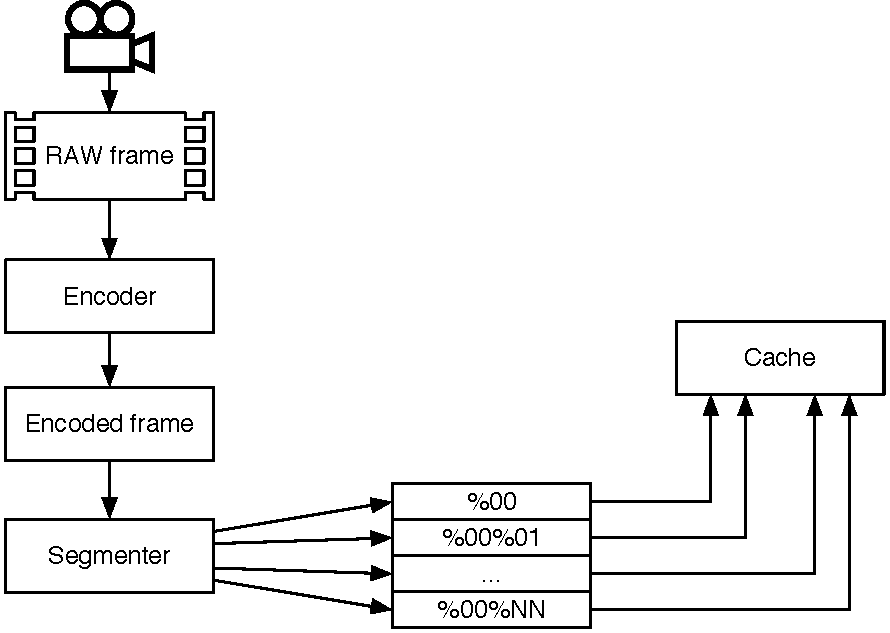
\includegraphics[width=0.4\textwidth]{producer}}\qquad
\subfigure[Consumer]{\label{fig:consumer}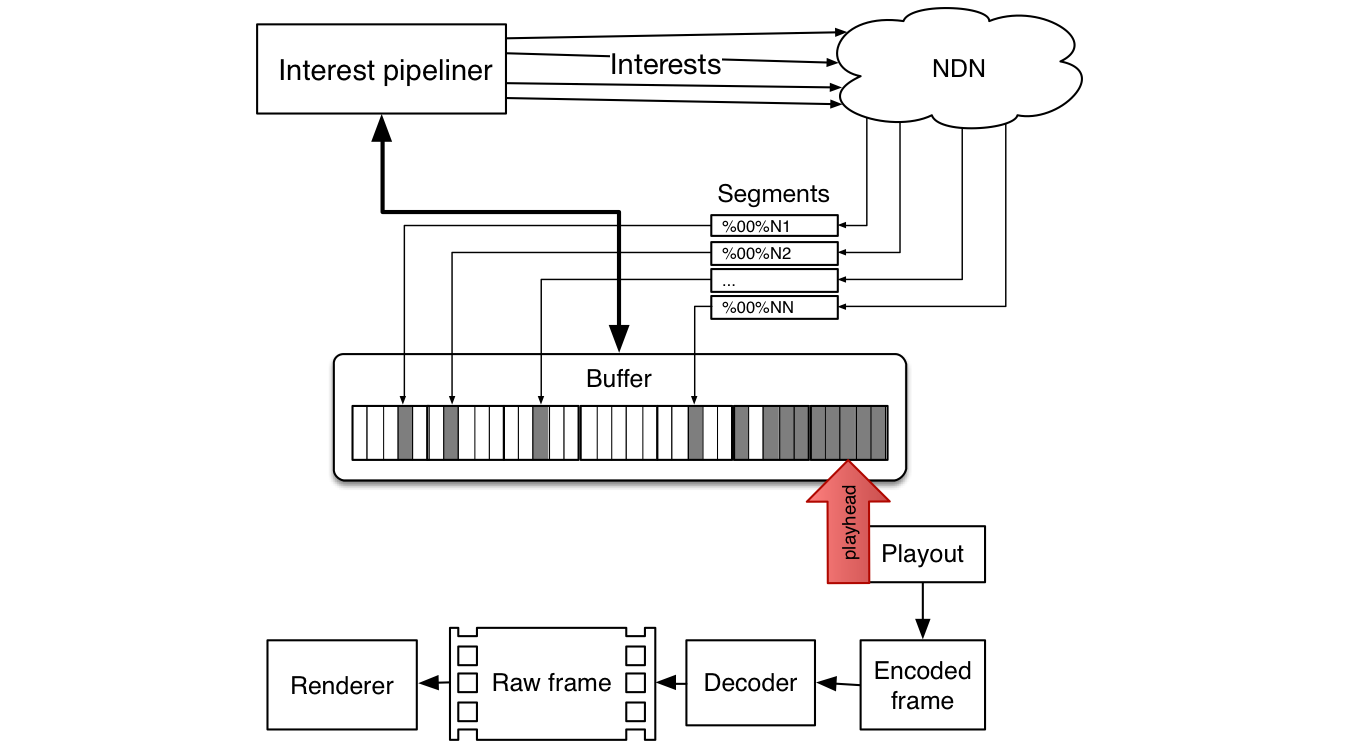
\includegraphics[width=0.4\textwidth]{consumer}}
\caption{\ndnrtcName{} producer and consumer operation.}
\end{figure}



There are two main roles defined in \ndnrtcName{}: producer and consumer. With NDN, the paradigm of real-time communication shifts from push-based (when the producer writes data to the socket, and the consumer reads it as fast as possible) to pull-based (the producer publishes data on the network at own pace, while the consumer has to request data needed and manage incoming data segments).

% Redundant figure
%
%\begin{figure}[t!]
%\centering
%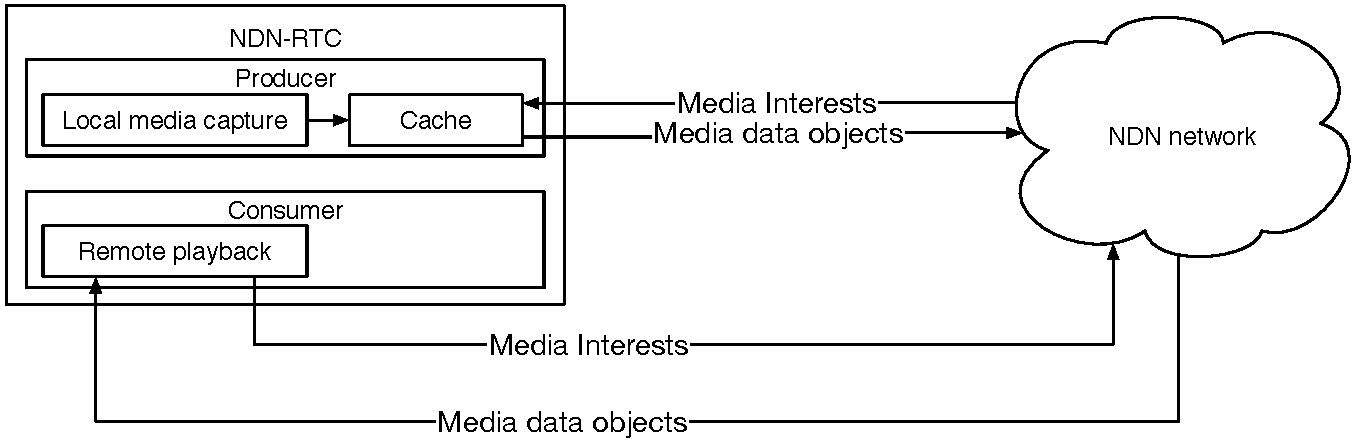
\includegraphics[width=0.5\textwidth]{architecture}
%\caption{RTC over NDN}
%\label{fig:arc}
%\end{figure}

Figure \ref{fig:arc} presents a top-level overview of how \ndnrtcName{} works. Local media capture and cache belong to the producer. Media is stored in the cache which provides access to the data for all incoming interests. Remote playback represents the consumer: issues interests, prepares received media (assembles video frames from segments and re-orders them) and plays it back.

\subsection{Producer}
The producer's main tasks are to acquire video and audio data from media inputs, encode them, pack them into network packets, and store them in the cache for incoming Interests. In this way, complexity shifts to the consumer, and scaling is supported by the network.

In the case of video streaming, the producer uses video encoding in order to reduce size of the frames. There are two types of encoded frames: \textit{Key} and \textit{Delta}. Key frames contain most of the video information, and do not depend on any previous frames to be decoded. Whereas Delta frames are dependent on the previous frames (received after the last Key frame), and cannot be decoded without significant visual artifacts if any of the Key frames are missing.

Encoded frames vary in size, but average bitrate stays the same. For example, the average sizes of frames for 1000 kbps stream using VP8/VP9: Key frames are $\approx$ 30KB, and delta frames are $\approx$ 3-7KB.
Therefore, depending on the underlying Internet Protocol used (IP in the existing NDN testbed), the producer may need to segment encoded frames into smaller chunks and provide clear naming conventions for the consumer to fetch them.




%************************************************
\subsection{Namespace}

As there is no direct consumer-producer communication, it is the producer's job to provide as much supportive information as possible, so that the consumer is able to use this information. These kinds should be reflected in the namespace:
media data (segmented video frames and bundled audio samples), error correction data, and metadata. 

%Besides that, the namespace should also reflect data specialization hierarchy - from general concepts in the root to more specialized entities towards the leaves. 

\subsubsection{Media} 

The \ndnrtcName{} producer uses a \textit{media stream} concept for describing published media. Media stream represents a flow of raw media packets (video frames or audio samples) coming from an input device. Streams usually derive names from their input devices. It is quite natural for a producer to publish several media streams simultaneously, if there is more than one device from which to publish media (for instance, video from camera, audio from microphone, and another video stream for computer screenshots). As all raw data should be encoded, the next level in the name hierarchy represents different encoder instances called \textit{media threads}. Thus, media threads allow the producer to provide the same media stream in several copies (for instance in low, medium and high quality, so that the consumer can choose media thread more suitable for current network conditions).

%\begin{figure}[t!]
%\centering
%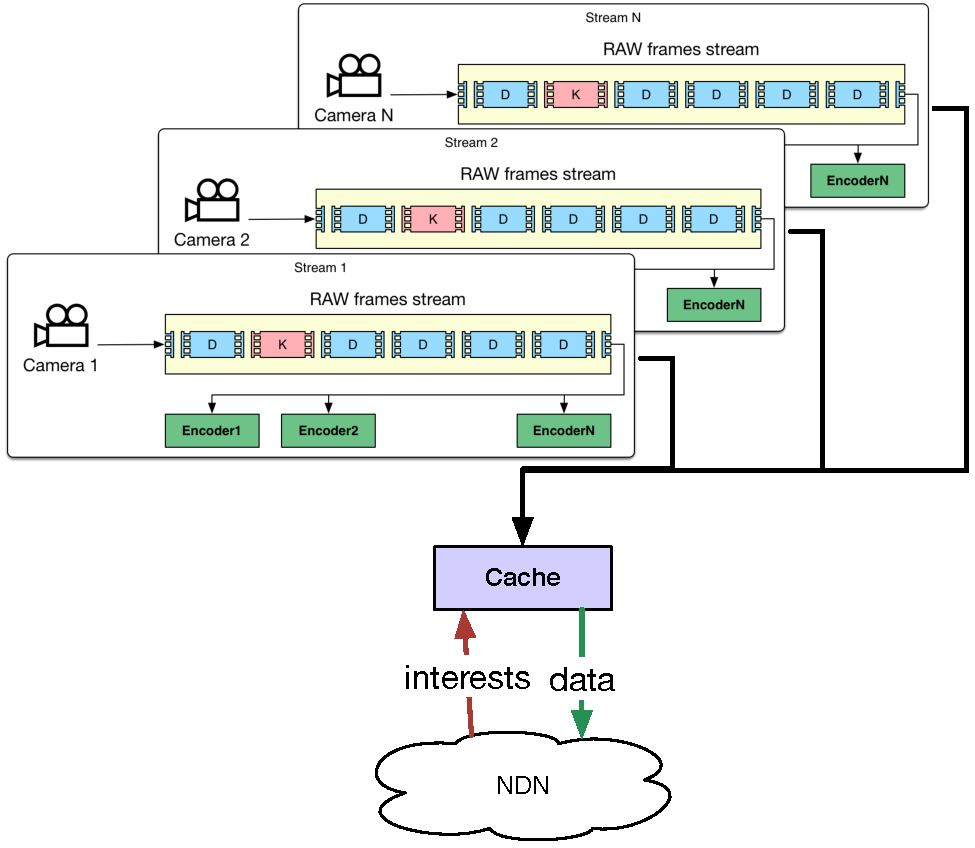
\includegraphics[width=0.5\textwidth]{streams-hierarchy}
%\caption{\ndnrtcName{} media streams hierarchy}
%\label{fig:stream-hierarchy}
%\end{figure}

\ndnrtcName{} does not use any specific media container format for delivering media to consumers. Instead, encoded media packets are segmented if needed and published under distinctive hierarchical names. Video frames are separated into two domains as per frame type, \textit{delta} and \textit{key}, and numbered sequentially and independently. Sequence numbers for both delta and key frames start from 0. Next level specializes data type, either media data or parity. Parity data, if the producer opts to publish it, can be used by a consumer to recover frames that miss one or more segments. The topmost level of the namespace defines individual data segments. These segments are also numbered sequentially, and segment numbers conform to NDN naming conventions \cite{ndn_naming}.

In the case of audio streams, there are some differences. First, there are no key frames; therefore all audio packets are published under the \textit{delta} namespace. Second, audio samples are significantly smaller than video frames and do not require to be segmented. In practice, it appears that multiple audio samples can be bundled into one data segment. Instead of segmenting audio packets, they are bundled together until the size of one data segment is reached, and published only after that.

Consumers need to know the producer's streams structure in order to fetch data successfully. In order to save consumers from traversing the producer's namespace, which can be time-consuming and unreliable, the producer publishes meta information about current streams under \textit{session info} component. Thus, consumers can retrieve up-to-date information about the producer's state.

\begin{figure}[t!]
\centering
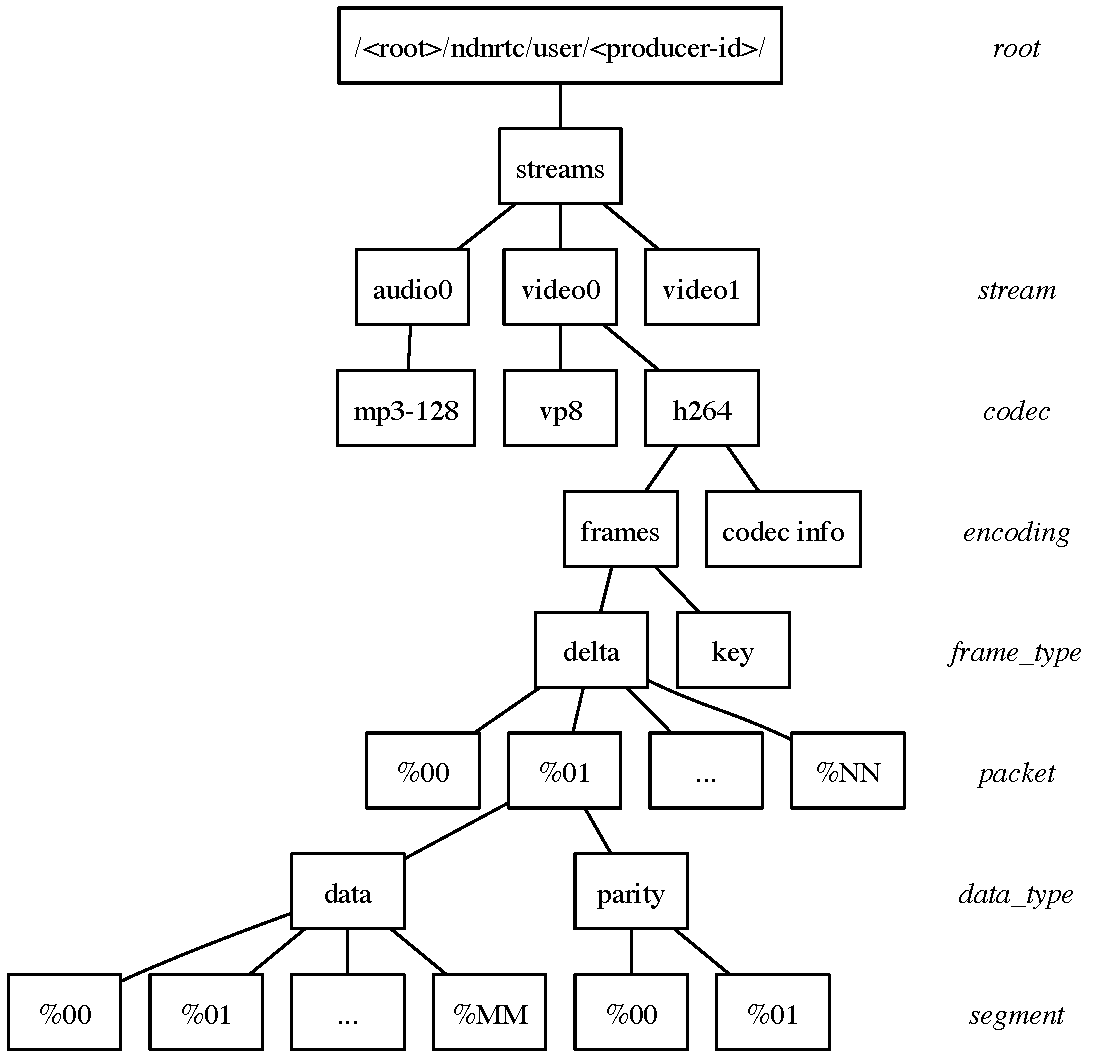
\includegraphics[width=0.45\textwidth]{namespace}
\caption{\ndnrtcName{} namespace}
\label{fig:namespace}
\end{figure}

\subsubsection{Metadata} 

Besides naming data objects, data names can be appended by some additional media-level meta information, which can be utlilized by consumers regardless of which frame segment was received first. Three components are added at the end of every data segment name:
\small\begin{equation}
.../\textbf{segment\#}/\textbf{playback\#}/\textbf{paired\_seq\#}/\textbf{num\_parity} \nonumber
\end{equation}\normalsize
\begin{itemize}[label={}]
\item \textit{playback\#} - absolute playback number for current frame; this is different from the \textit{frame\#} which is a sequential number for the frame in its domain (i.e. Key or Delta);
\item \textit{paired\_seq\#} - sequential number of the corresponding frame from other domain (i.e., for delta frames, it is sequential number of the corresponding key frame which is required for decoding);
\item \textit{num\_parity} - number of parity segments for particular frame.
\end{itemize}

The pull-based nature of NDN and our experimental application's deliberate avoidance of explicit consumer-producer synchronization (allowing publisher-independent scaling) have shown the importance of providing sufficient meta information on the producer side. Such information (which could include Interests' nonce values, Interests' arrival timestamps and data generation delays), if added to the returned data segment, may help consumers evaluate relevant network performance, detect congestion and assess whether incoming data is likely to be stale (delayed beyond the path delay). Furthermore, keeping historical data on the consumer side may help Interest pipelining in the future. For instance, providing the average number of segments per frame type helps consumers estimate the number of required initial Interests to fetch upcoming frames. This helps keep frame fetching cycles minimal.


%************************************************
\subsection{Data objects}
Producer generates signed data objects from input media streams and places them in cache instantly. Incoming Interests retrieve data from cache, if it is present, or forward further to the producer, if the requested data has yet to be produced. In such cases, the producer maintains a pending Interests table (PIT), which is checked every time a new data object is generated. If an Interest for a newly generated data object exists in the PIT, it gets answered, and PIT entry is erased.

\subsubsection{Media stream}
%% TODO: What's the media payload? 

\begin{figure}[t!]
\centering

\subfigure[video frame segmentation]{\label{fig:segment}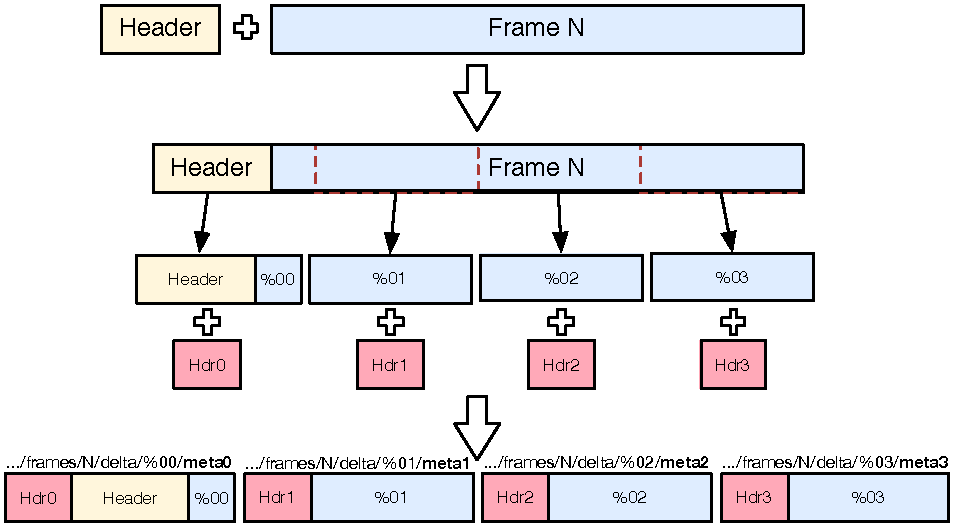
\includegraphics[width=0.5\textwidth]{segmentation}}
\subfigure[audio samples bundling]{\label{fig:audio-bundling}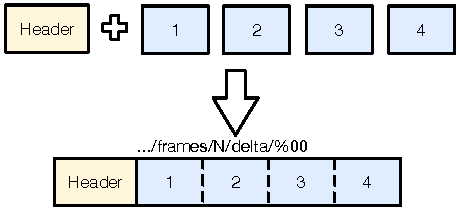
\includegraphics[width=0.3\textwidth]{audio-bundling}}

\caption{Segmentation and bundling}

\end{figure}

\subsubsection{Metadata}

Besides actual stream data, data objects contain some amount of meta information which is prepended during frames segmenting (see Figure \ref{fig:segment}). There are two header types: \textit{Frame header} and \textit{Segment header}. Frame header is prepended to segment \#0 of each individual video frame, and contains media-specific information (such as size of a frame), timestamp, current rate and unix timestamp, which can be used for calculating actual delay between NTP-synchronized producer and consumers (see Figure \ref{fig:data-struct}). Segment header is prepended to every segment of a frame. It carries network-level information which can be used by consumers to estimate current network conditions and origin of the data objects received:
\begin{itemize} [label={}]

\item \textit{Interest arrival timestamp}: Timestamp of the interest arrival. Monitoring this value and interest expression timestamps over time may give consumers a clue about how it takes for Interests to reach the producer. This value is only valid when nonce value belongs to one of a given consumer's Interests.

\item \textit{Generation delay}: Time interval in milliseconds between Interest arrival and segment publishing. A consumer can use this value in order to control the number of outstanding Interests. This value is only valid when nonce value belongs to one of the consumer's Interests.

\item \textit{Interest nonce}: Nonce value of the interest which requested this particular segment. There are three meaningful cases:  1) \textit{value belongs to the Interest issued previously} - consumer received non-cached data requested by Interest issued previously; 2) \textit{value is non-zero, but does not belong to any of the previously issued Interests} - consumer received data requested by some other consumer; data may be cached; 3) \textit{value is zero} - consumer received data which was cached on the producer side and never requested by anyone before.

\end{itemize}

\begin{figure}[t!]
\centering
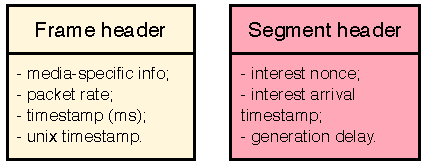
\includegraphics[width=0.3\textwidth]{data-struct}
\vspace{-4pt}
\caption{Frame and segment headers}
\label{fig:data-struct}
\end{figure}

Audio samples are not prepended by any segment header, however the whole audio bundle is prepended by the same frame header (see Figure \ref{fig:audio-bundling}).

%************************************************
\subsection{Consumer}

Consumer implements more sophisticated algorithms to achieve following goals:
\begin{itemize}
\item ensure fetching the latest data available in the network; 
\item choose appropriate media stream bandwiths provided by a producer, by monitoring network conditions;
\item playback fetched media in correct order;
\item handle network latency and packet drops.
\end{itemize}

The consumer takes into account that media packets are presented by separate segments in the network. Therefore, the consumer implements mechanisms of Interest pipelining and frame buffering (see Figure \ref{fig:consumer}). Interest pipeline issues Interests for individual segments, and is controlled by some higher-level logic which achieves one out of four consumer's goals. It ensures that only the latest data is fetched. Packets re-ordering, drops and latency fluctuations absorbtion are attained by the frame buffer, which introduces buffering delay and re-arranges received frames in the playback order.



%************************************************
\subsubsection{Frame fetching}

Consumers do not know the total number of segments beforehand, unless the very first segment is fetched. In this case, the consumer can retrieve metadata from the received segment and acquire total number of segments for the current frame. 
Therefore, at first attempt, the consumer tries to make a "best guess" at the number of segments needed to fetch, by issuing $M$ Interests (see Figure \ref{fig:pull}). If Interests arrive too early, they will be added to the producer's PIT and stay there for the amount of time $d_{gen}$ called \texttt{generation delay}. Once encoded frame is segmented into $N$ segments, these are published, and if $N\geq M$, Interests $0 - M$ are answered with the data which travels back to the consumer. Upon receiving first data segment, the consumer determines the total number of segments for the current frame, and issues $N - M$ more Interests for the missing segments (if any). These segments will be satisfied by data with no generation delay (as the frame has been published already by the producer). The time interval between receiving very first segment and when the frame is fully assembled is represented by $d_{asm}$ and called \texttt{assembling time}.

\begin{figure}[t!]
\centering
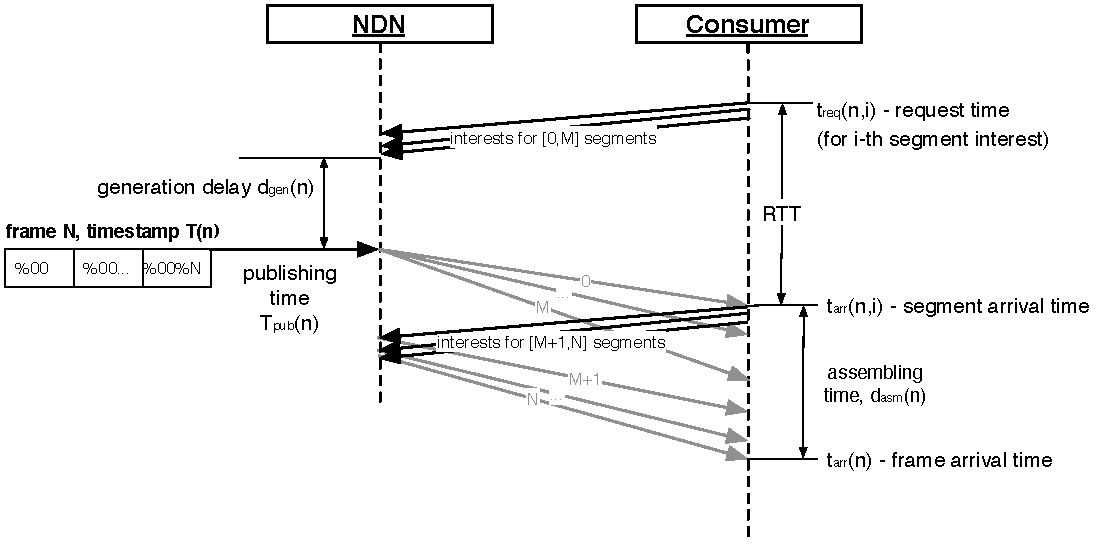
\includegraphics[width=0.5\textwidth]{frame-fetch}
\vspace{-18pt}
\caption{Fetching frame}
\label{fig:pull}
\end{figure}

Needless to say, additional round-trips for requesting missing data segments increase overall frame assembling time and chances that the frame will be incomplete by the time it should be played back. This problem could be avoided if the consumer is able to make better estimates of the number of initial Interests. Therefore, the following considerations were introduced in later versions of the library:
\begin{itemize}
\item consumer should know what type of frame is to be fetched (as average number of segments varies greatly for different frame types);
\item consumer should track average number of segments per frame type.
\end{itemize}

The first consideration was implemented by introducing separate namespaces for key and delta frames. The second consideration helps consumers better estimate the number of initial interests.

\subsubsection{Buffering}

% Buffer:
% - re-ordering
% - added latency to mitigate network delays
% - extended defition:
% 	- pending frames
% 	- assembling frames
% - buffer-based retransmissions

As in traditional streaming applications, consumer uses frame buffering in order to tackle out-of-order data arrivals and network delay deviations. Consumer-side jitter buffer is also used as a place for assembling frames by segments. However, the definition of jitter buffer is extended for NDN. In a traditional push-based approach, buffer can not contain empty frame slots; they are allocated/reserved only when data arrives. A pull-based paradigm requires consumers to request data explicitly. Therefore, after expressing an Interest, consumers "knows" that new data is coming, and a frame slot should be reserved in the buffer. Practically, this means that there will always be some number of reserved empty slots in the buffer. Thus, jitter buffer's size has two measurements:
\begin{itemize}[label={}]
\item \textit{playback size} - playback duration of all complete ordered frames by the moment;
\item \textit{estimated size} = \textit{playback size} + \textit{number of reserved slots} $\times$ 1/\textit{producer rate}.
\end{itemize}

The difference between estimated size and playback size ($RTT^{\prime}$) cannot be smaller than the current average RTT value. In fact, keeping this value at a minimum indicates that consumer receives the most recent data with the minimal amount of outstanding Interests. Monitoring this value over time may help consumer get a better clue on the ``sync" status with the producer. For example, consumer may use it during the fetching process, as will be discussed in the next section. 

\subsubsection{Interest expression control}

The key challenge in a consumer-driven model for videoconferencing is to \emph{ensure the consumer gets the latest data in a caching network}, without resorting to direct producer-consumer communication that would limit scaling. To get fresh data, which can be cached but should not be the newest available for the consumer's path,  the consumer cannot rely only on using such flags as \textit{AnswerOriginKind} and \textit{RightMostChild}. The high frequency nature of streaming data makes no guarantees that the data satisfying those flags received by a consumer will be the most recent one. Instead, it is necessary to use other indicators to ensure that the network supplies up-to-date stream data. The basic solution is to leverage the known segment publishing rate and assume, under normal operation, that a series of old, cached samples can be retrieved more quickly than new data. The inter-arrival delays ($D_{arr}$) of the most recent samples follow the publishers' generation pattern, but cached data will follow the Interest expression temporal pattern. Therefore, by monitoring inter-arrival delays of consequtive media samples, consumers can make educated assumptions about data freshness (see Figure \ref{fig:inter-arrival}).

\begin{figure}[t!]
\centering

\subfigure[bursty cached data arrival, reflects interests expression pattern]{\label{fig:cached}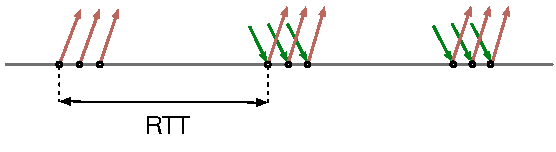
\includegraphics[width=0.4\textwidth]{arrival-cached}}\\
\subfigure[stable fresh data arrival, reflects publishing pattern]{\label{fig:fresh}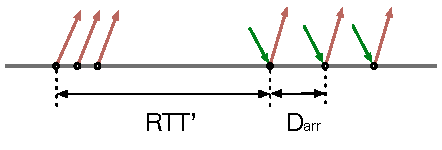
\includegraphics[width=0.35\textwidth]{arrival-fresh}}

\caption{Getting the latest data: arrival patterns for the cached and most recent data}
\label{fig:inter-arrival}
\end{figure}

During bootstrapping, the consumer ``chases" the producer and aims to exhaust network cache of historical (non-real time) segments. By increasing the number of outstanding Interests, the consumer ``pulls cached data" out of the network, unless the freshest data begin to arrive. In order to control Interest expression, a concept of $W$ (roughly an ``Interest window") is introduced (see Figure \ref{fig:w-concept}). It expresses Interests only when $W > 0$. At every moment, $W$ indicates how many outstanding Interests can be sent. Before the bootstrapping phase, the consumer initializes $W$ with a value which reflects the consumer's estimate of how many Interests are needed in order to exhaust network cache and reach the most recent data. 

\begin{figure}[t!]
\centering

\subfigure[$W$ concept]{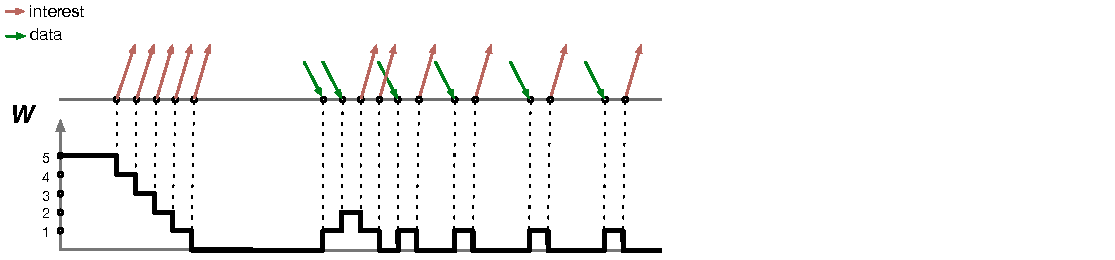
\includegraphics[width=0.35\textwidth]{w-concept}}
\subfigure[interests bursting ($W+3$)]{\label{fig:int-burst}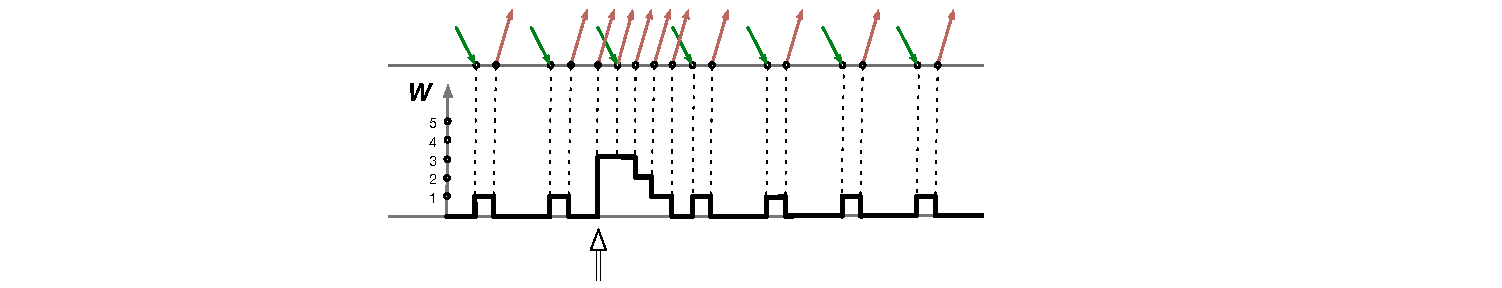
\includegraphics[width=0.35\textwidth]{int-burst}}
\subfigure[interests withholding ($W-3$)]{\label{fig:int-hold}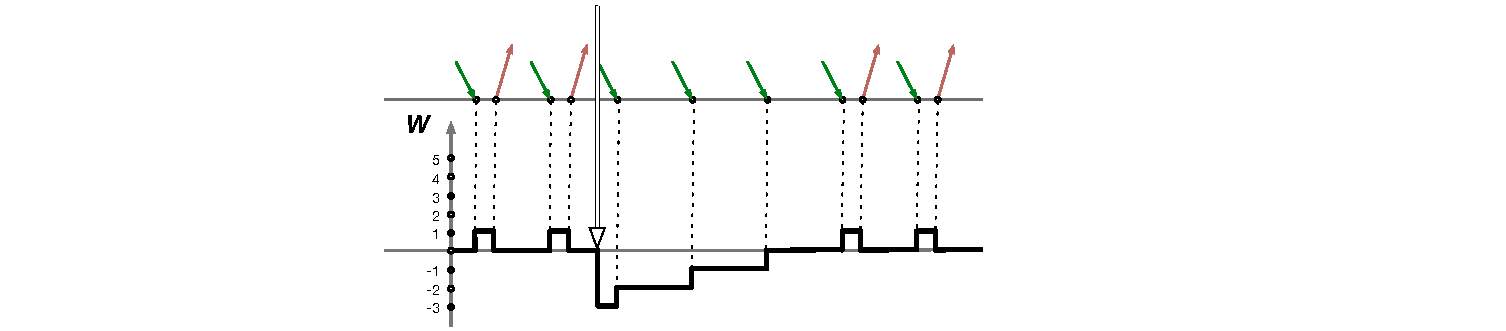
\includegraphics[width=0.35\textwidth]{int-hold}}

\caption{Managing interest expression}
\label{fig:w-concept}
\end{figure}


$W$ provides a simple mechanism to speed up or slow down Interests expression. Any increase in $W$ value makes consumer issue more Interests (Figure \ref{fig:int-burst}), whereas decrease in $W$ holds consumer back from sending any new Interests (Figure \ref{fig:int-hold}). Larger values of $W$ make consumer reach synchronized state with the producer more quickly. However, a larger value means a larger number of outstanding Interests and larger $RTT^\prime$ because of longer generation delays $d_{gen}$ for each media sample. By adjusting the value of $W$ and observing inter-arrival delays $D_{arr}$ consumer can find minimal $RTT^\prime$ value while still getting non-cached data, thus achieving best synchronization state with the producer.

For more complex scenarios of video streaming, the consumer controls expression of ``batches" of Interests rather than individual Interests, because video frames are composed of several segments. In this case, $W$ is adjusted on a per-frame basis, rather than per-segment. In all other respects, the same logic (as above) can be applied.

The bootstrapping phase starts with issuing Interest with enabled \textit{RightMostChild} selector, in delta namespace for audio and key namespace for video. The reason this process differs for video streams is that consumer is not interested in fetching delta frames without having corresponding key frame for decoding. Once initial data segment of sample with number $S_{seed}$ has been received, consumer initializes $W$ with initial value $N$ and asks for the next sample data $S_{seed}+1$ in the appropriate namespace. Upon receiveing first segments of sample $S_{seed}+1$, consumer initiates fetching process (described above) for all namespaces (delta and key, if available). This bootstrapping phase stops when consumer finds the minimal value of $W$ which still allows receiving the most recent data, i.e., consumer reaches synchronized state with the producer and switches to a normal fetching phase where no adjustments for $W$ are needed. 
% Listing \ref{lst:fetch-algo} shows pseudo-code for the bootstrapping phase.

% \begin{algorithm}
% \begin{algorithmic}

% \Function{Bootstrap}{Meta}

% \If {audio}
% 	\State $Nspc \gets DeltaNamespace$
% \Else
% 	\State $Nspc \gets KeyNamespace$
% \EndIf

% \State \Call{ExpressOne}{$RightMostChild$, $Nspc$}
% \Ensure Received data segment $Dseed$
% \State $Sseed \gets$\Call{GetSeqNumber}{$Dseed$}
% \State $NavgKey \gets$\Call{GetAvgSegNum}{$Meta$, $Key$}
% \State \Call{ExpressBulk}{$NavgKey$, $Sseed+1$, $Nspc$}
% \Ensure Received data segment $D$ for $Sseed+1$
% \State $J \gets$ \Call{GetDeltaNumber}{$D$}
% \State $NavgDelta \gets$\Call{GetAvgSegNum}{$Meta$, $Delta$}
% \State $DW \gets N$
% \State $W \gets DW$

% \While{$BootstrappingPhase$}

% \While{$W > 0$}
% 	\State \Call{ExpressBulk}{$NavgDelta$, $J$, $Delta$}
% 	\State $W \gets W-1$
% 	\State $J \gets J+1$
% \EndWhile

% \If {received segment $Dj$ for new sample}
% 	\State $W \gets W+1$
% \EndIf

% \EndWhile

% \State \Call{Switch}{$FetchingPhase$}

% \EndFunction

% \end{algorithmic}

% \label{lst:fetch-algo}
% \caption{Bootstrap}
% \end{algorithm}


%\subsubsection{Application-level PIT}
\textit{Application-level PIT.} In most cases, consumers aim to express Interests for the data not yet produced, to be immediately satisfied when data is produced. The current NDN-CPP library provides a producer-side Memory Content Cache implementation into which data is published. However, this is only useful when data has been published and put in the cache before Interest for this data has arrived. For the missing data, the Interest is forwarded to the producer application which stores it in internal pending interests table (PIT) unless requested data is ready. This functionality seems quite common for low-latency applications, and has now been incorporated into the NDN-CPP library implementation.

\section{Implementation}
\label{sec:imp}
\ndnrtcName{} is implemented as a library written in C++, which is available at \url{https://github.com/remap/ndnrtc}. 
It provides publisher interface for publishing arbitrary number of media streams (audio or video), and consumer interface with a callback for rendering decoded video frames in a host application. OS X platform is currently supported; Linux build instructions will be added soon. 
The library distribution also comes with a simple console application which demonstrates the use of \ndnrtcName{} library.

\ndnrtcName{} exploits some functionality from several third-party libraries it is linked against with: NDN-CPP \cite{ndnccl} is used for NDN connectivity. The WebRTC framework \cite{webrtc} is utilized in two ways: 1) incorporation of the existing video codec; 2) full incorporation of the existing WebRTC audio pipeline, including echo cancellation;  3) OpenFec \cite{openfec} library is utilized for forwad error correction support.

Apart from the library, first desktop NDN videconferencing application \ndnconName{} \cite{ndncon} was implemented atop \ndnrtcName{}. It provides convenient UI for publishing and fetching media streams, text chat and organizing multi-party audio/video conferences.

\section{Evaluation}
\label{sec:eval} 
In the course of this project, there were several iterations of architecture design that introduced successive improvements to the overall quality of the algorithms. They are described further in this section. Each iteration tackles problems revealed during tests, which were mostly taken in practice rather than simulated.

\subsection{Key namespace}
As was described in previous sections, Key frames are usually much heavier than Delta frames and require more data segments for delivery. In early library versions, this differentiation was not reflected in producer's namespace which made consumer to pipeline equal number of initial interests ($M$ on Figure \ref{fig:pull}) for both frame types. This resulted in larger assembling times ($d_{asm}$) for the Key frames and additional round-trips of missing interests. Increased assembling time quite often caused skipping incomplete Key frames as they were not assembled by the time they should be played out. Eventually, all the consequent Delta frames were skipped as well which degraded overall video streaming experience by introducing video ``hiccup" effect.

Having separate namespace for Key frames allowed consumer to maintain separate interest pipelines per frame time and collect historical data on the average number of interests required to fully retrieve one frame of each type in one round trip.

\subsection{Audio bundling}
\begin{figure}[t!]
\centering
\begin{tiny}
\def\svgwidth{0.5\textwidth}\input{tests-skype.pdf_tex}
\end{tiny}
\vspace{-18pt}
\caption{2-peer conference tests compared to Skype}
\label{fig:tests-skype}
\end{figure}

A series of tests were taken in order assess efficiency and quality of service compared to Skype calls. Each test was comprised of six runs of 2-person 5-minute conference talks using NdnCon (GUI conferencing application build atop \ndnrtcName{}):
\begin{itemize}
\item 3 runs of audio+video on low, medium and high qualities (0.5, 0.7 and 1.5 Mbit/s accordingly);
\item 1 run of audio-only;
\item 1 run of Skype audio+video conference;
\item 1 run of Skype audio only conference.
\end{itemize}

Tests were taken across existing NDN testbed between REMAP hub (aleph.ndn.ucla.edu) and six other hubs. Therefore, tests were covering both one-hop and multi-hop topologies.

Figure \ref{fig:tests-skype} shows overall bitrate usage results. Firstly, whereas Skype has fully utilized link capacity between peers and delivered higher bitrate videos, NdnCon did not adjust to the current network conditions which makes feature of adaptive rate control highly desirable.

Actual average bitrates are turned out to be slightly higher than pre-configured video streams (0.7, 0.9 and 1.8 Mbit/s) which can be explained by NDN packet overhead which is about 280-330 bytes large and account for $\approx$30\% of segment size (1000 bytes). Having such large overhead makes transferring audio samples in separate segments highly inefficient. Thus, further improvent to the algorithms was to bundle consecutive audio samples unless they fill the size of a segment. With 90 Kbit/s audio, approximately 5 audio samples can be added to 1000-bytes data segment. This improvement eventually reduced audio bandwith efficiently (and interests number on consumer side) and made it comparable to Skype ausio bandwiths.

\subsection{Consumer-Producer synchronization}

\begin{figure}[t!]
\centering
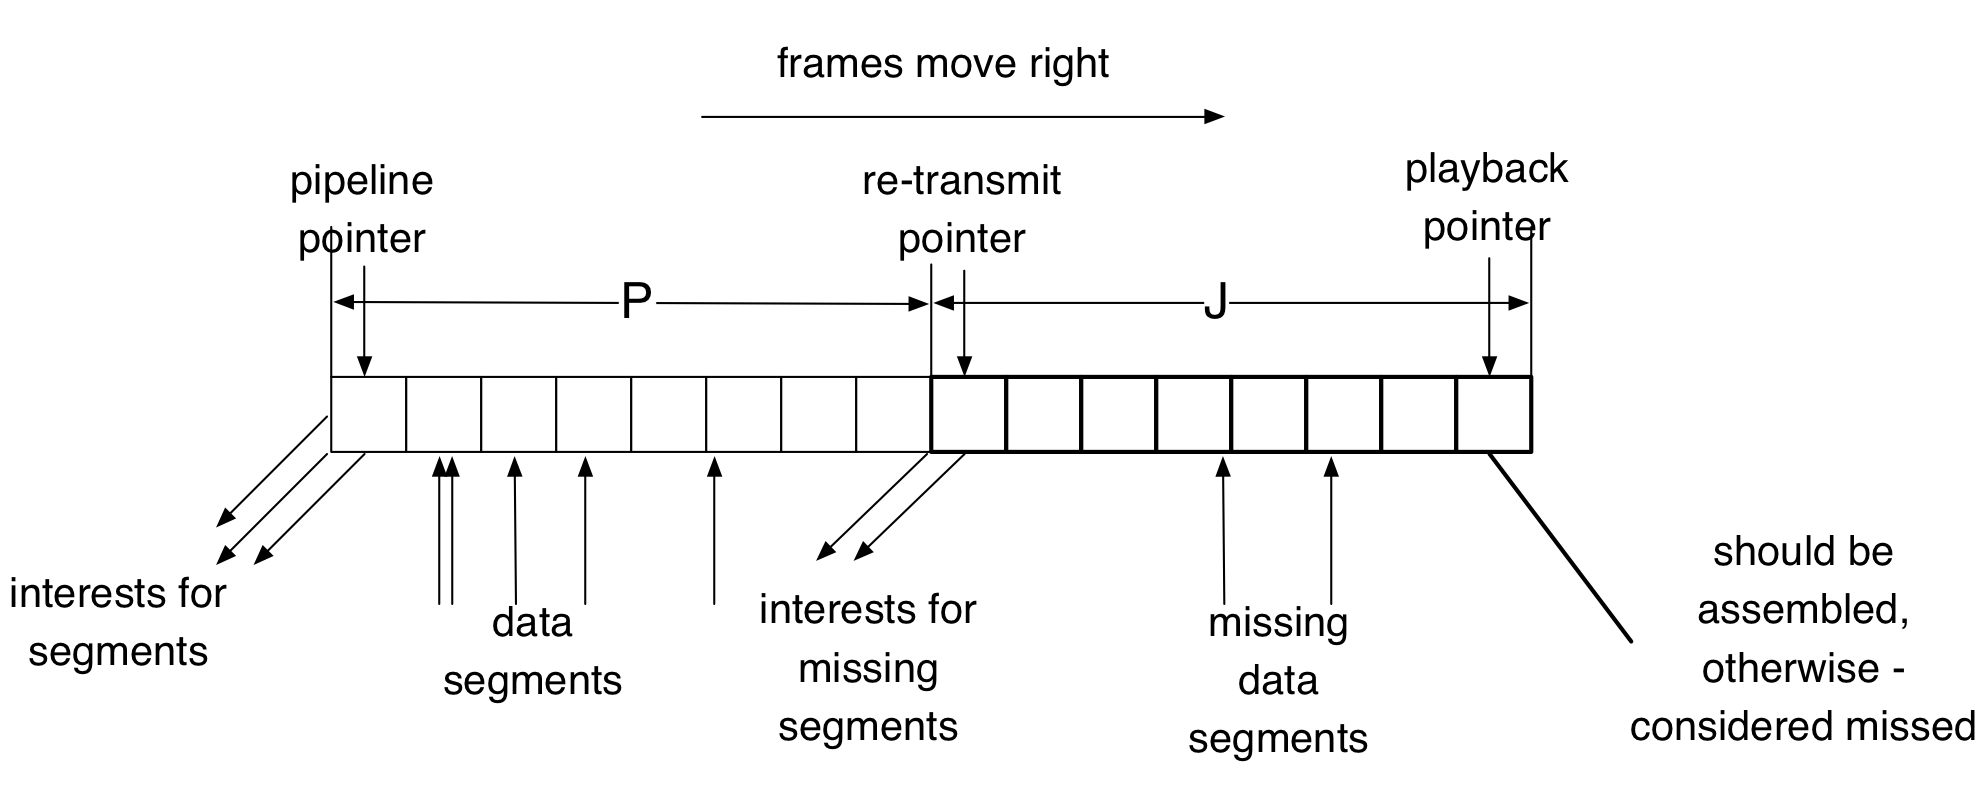
\includegraphics[width=0.5\textwidth]{buffer}
\caption{Bufferization in earlier library versions}
\label{fig:old-buf}
\end{figure}

In previous library versions, the consumer ``chased" the producer's time-series data by exhausting cached data and issuing large number of outstanding interests. However, there were no mechanism for consumer to figure out how early those interests are issued and whether interest expression should be postponed in order to eliminate timeouts. For two similar test runs (one-hop topology) the number of timed out interests and retransmissions could vary greatly (either $\approx$1\% or $\approx$50\%). The latter case happened due to incorrect consumer's synchronization with the producer - interests were issued too early so that they were timed out before any data has been produced. This problem could be solved by increased interests' lifetime. However, for previous library versions, bufferization mechanism (see Figure \ref{fig:old-buf}) dictated interests' lifetime - in fact, in order to maintain re-transmission checkpoint, all interests entering the buffer should have lifetime equals half of the current buffer size. This approach resulted in unavoidable interests time outs in cases when consumer issued interests far too early before the actual data was produced.

For the current version of the library, re-transmission check-point is placed at $RTT$ milliseconds from the end of the buffer ($J=RTT$ on the Figure \ref{fig:old-buf}), this, together with updated NFD retransmission streategy \cite{nfd-rtx}, alllowed larger interests lifetimes.

Moreover, the problem described above could not have happened if consumer would know that it issues interests too early. Chasing algorithm in older library versions was exhausting network cached in rather aggressive manner - interests were issued constantly unless they fill up the buffer. After that, frames would be consumed at the producer's rate and more interests issued unless consumer reaches stable data arrivals. This approach lacks from any knowledge about issued interests and generation delay or $RTT`$ is not taken into account.

\begin{figure}[t!]
\centering
%\captionsetup[subfigure]{aboveskip=-1pt,belowskip=-2pt}
\begin{scriptsize}
\subfigure[$W=10$: short chasing, larger $RTT^\prime$]{\def\svgwidth{0.48\textwidth}\input{w10.pdf_tex}}
\subfigure[$W=4$: longer chasing, smaller $RTT^\prime$]{\def\svgwidth{0.48\textwidth}\input{w4.pdf_tex}}
\subfigure[$W=3$: consumer can't exhasut cache, $RTT^\prime = RTT$]{\def\svgwidth{0.48\textwidth}\input{w3.pdf_tex}}
\end{scriptsize}
\caption{Larger $W$ decreases ``chasing" phase, but increases $RTT^\prime$ for the same network configuration ($RTT\approx100ms$)}
\label{fig:ws}
\end{figure}

With introduction of $W$ concept, consumer have full control of the interest expression. Figure \ref{fig:ws} shows how bigger value of $W$ helps to exhaust cache faster. The number of outstanding interests is controlled by a consumer and directly influences how fast consumer can ``chase" the producer. Every time a new interest is expressed, $W$ gets decremented and when new data arrives, $W$ is incremented, thus allowing consumer to issue more interests. $W$ concept allows "lazy" start for consumer - by specifying smaller $W$, consumer issues less interests. Further, consumer observes cache exhaustion by monitoring $D_{arr}$ and, if cache has not been exhausted during allocated time, consumer may increase the value of $W$ in order to express more interests. Similarly, consumer may opt to decrease $W$ in cases where original value resulted in too agressive behaviour.

%\subsection{Test setup} 

%Include testbed topologies used, collaboration with WUSTL

%- one-hop
%- multiple-hops
%- many-to-many conferencing

%\subsection{Quality of experience} 

%How was the end-user quality of experience by the time the paper was written
%What kinds of things did you add to support it. 

\subsection{Scaling}

For now, there were few multi-peer tests conducted using NdnCon. The maximum number of participants involved in audio/video conference was four people, who were spread out accross 4 different campuses.

\section{Conclusion and Future Work}
\label{sec:conclusion}


\begin{figure}[t!]
\centering
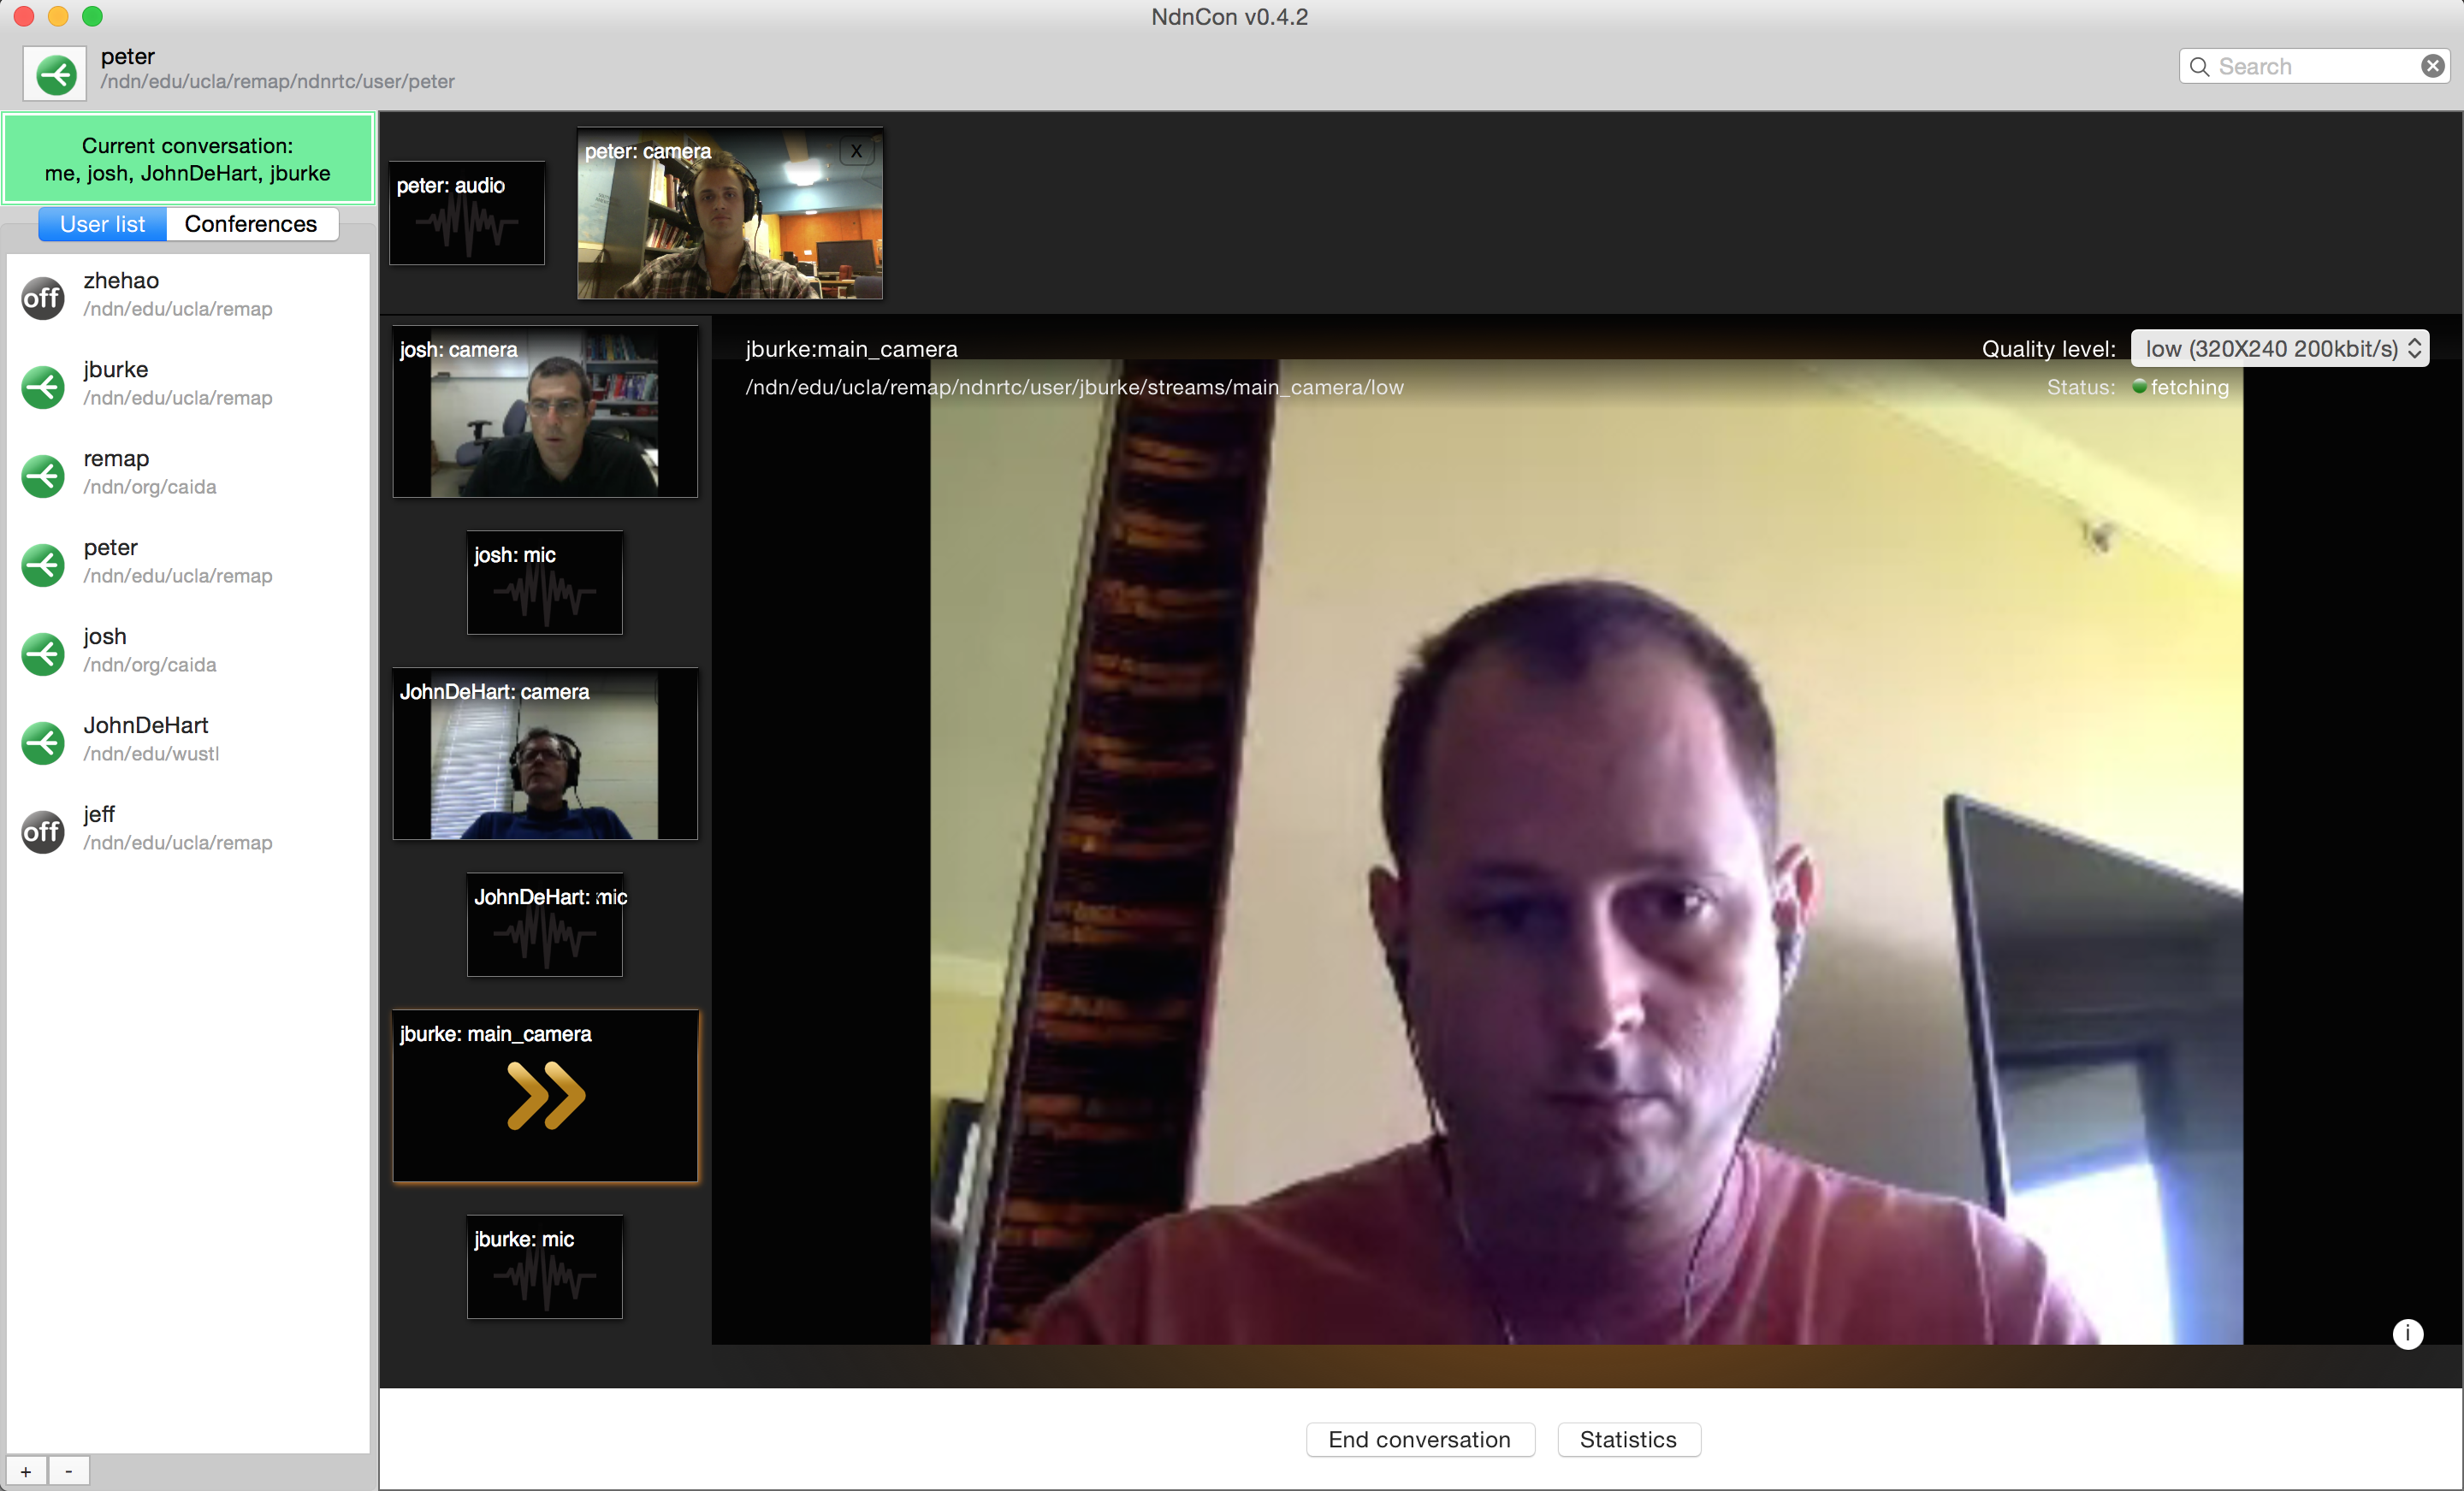
\includegraphics[width=0.3\textwidth]{ndncon}
\caption{\ndnconName{} screenshot [@@REPLACE]}
\label{fig:ndncon}
\end{figure}

%% TODO: Conclusion

Discuss quality of experience. 

Future work: 
\begin{itemize}[label={}]
\item \textbf{Adaptive rate control.} In the current library design, the producer may deliberately choose to publish several copies of the same video stream with different encoding parameters, thus allowing consumer to select the most appropriate stream for current network conditions. However, the selection is made manually and depends on user's perceptual assessment of the retrieved media. Implementation of adaptive rate control would simplify this process, and allow the network to be utilized more efficiently based on current conditions.

\item \textbf{Scalable video coding.} An elegant way to offload the producer from publishing multiple copies of the same video stream in different bandwidths is to utilize Scalable Video Coding. By reflecting SVC layers in the namespace, consumer will have more freedom for adapting media streams to the current network. This opportunity should be explored and added in a future versions.

\item \textbf{Encryption-based access control} The current \ndnrtcName{} design supports basic content signing and verification. However, further basic security features have yet to be implemented, e.g., media data encryption, consumer access control.

\item \textbf{Conference management} 
Work on ndncon. unknown but verified publishers trust; 
\end{itemize}
%%signatures consistency checks for successive media packets 
%% need to add the above before publication %%;  


\section{Acknowledgements}
\label{sec:Acknowledgements}
This project was partially supported by the National Science Foundation (award CNS-1345318 and others) and a grant from Cisco. The authors thank Lixia Zhang, Van Jacobson, and David Oran, as well as Eiichi Muramoto, Takahiro Yoneda, and Ryota Ohnishi from Panasonic Research, for their input and feedback. John DeHart, Josh Polterock, Jeff Thompson, and others on the NDN team provided invaluable testing of \ndnconName{}.  The initial forward error correction approach in \ndnrtcName{} was by Daisuke Ando. 

\bibliographystyle{abbrv}
\bibliography{bibliography}


\end{document}